\documentclass[12pt,a4paper]{article}
\usepackage[utf8]{inputenc}
\usepackage[OT1]{fontenc}
\usepackage{amsmath}
\usepackage{amsfonts}
\usepackage{amssymb}
\usepackage{graphicx}
\usepackage{tikz}
\usepackage{pgfplotstable}
\usepackage{mathtext}

\usepackage[T1]{fontenc}
\usepackage[utf8]{inputenc}
\usepackage[english, bulgarian, russian]{babel}

\usepackage{tikz}
\usepackage{pgfplots}
\usepackage{indentfirst}
\usepackage[export]{adjustbox}
\usepackage{multirow}
\usepackage{geometry} \geometry{verbose,a4paper,tmargin=2cm,bmargin=2cm,lmargin=1.5cm,rmargin=1.5cm}

\graphicspath{{Images/}}
\usepackage[left=2cm,right=2cm,top=2cm,bottom=2cm]{geometry}
\usepackage{wrapfig}
\usepackage{setspace}
\usepackage{indentfirst}
\usepackage{subfigure}


\begin{document}

\begin{titlepage}
  \begin{center}
    \huge
    Московский Физико-технический Институт
    
    (Национальный исследовательский университет)
    \vspace{0.5cm}

   
    \vspace{0.25cm}
 
    \vfill
 
    \vfill

    \textsc{\bf{Отчет о выполнении работы 2.1.4}}\\[3mm]
    
    {\LARGE  Определение теплоемкости твердых тел}
  \bigskip
    \vfill
    
\end{center}
\vfill
\begin{flushright}

    Выполнили студентки 1 курса
    
    ФБМФ, группа Б06-103

    Попеску Полина
    
    
    Фитэль Алёна

\end{flushright}
\bigskip


\vfill

\begin{center}
  Долгопрудный, 2022 г.
\end{center}
\end{titlepage}

\section{Введение}

	\textbf{Цель работы:} измерение количества подведенного тепла и вызванного им нагрева твердого тела; определение теплоемкости по экстраполяции отношения $\Delta Q / \Delta T$ к нулевым потерям тепла.

	\textbf{В работе используются:} калориметр с нагревателем и термометром сопротивления; амперметр; вольтметр; мост постоянного тока; источник питания 36 В.

\section{Теоретический материал}


Теплоемкость определяется по формуле
\begin{equation}
	C = \frac{\Delta Q}{\Delta T},
	\label{eq:dQdT}
\end{equation}

где $\Delta Q$ -- количество тепла, подведенного к телу, и $\Delta T$ -- изменение температуры тела, произошедшее в результате подвода тепла.

Температура исследуемого тела надежно измеряется термометром сопротивления, а определение количества тепла, поглощенного телом, обычно вызывает затруднение. В реальных условиях не вся энергия $P \Delta t$, выделенная нагревателем, идет на нагревание исследуемого тела и калориметра, часть ее уходит из калориметра благодаря теплопроводности его стенок. Оставшееся в калориметре количество тепла $\Delta Q$ равно 
\begin{equation}
	\Delta Q = P\Delta t - \lambda(T - T_{\text{к}}) \Delta t,
	\label{eq:dQ}
\end{equation}
где $P$ -- мощность нагревателя, $\lambda$ -- коэффициент теплоотдачи стенок, $T$ -- температура тела, $T_{\text{к}}$ -- комнатная температура, $ \Delta t$ -- время, в течение которого идет нагревание.

Из уравнений (1) и (2) получаем
\begin{equation}
    C = \frac{P - \lambda(T - T_{\text{к}})}{\Delta T / \Delta t}
    \label{osnovnaya}
\end{equation}
Формула (3) является основной расчетной формулой. Она определяет теплоемкость тела вместе с калориметром. Теплоемкость калориметра измеряется отдельно и вычитается из результата.

С увеличением температуры исследуемого тела растет утечка энергии, связанная с теплопроводностью стенок калориметра. Из формулы (2) видно, что при постоянной мощности нагревателя по мере роста температуры количество теплаб передаваемое телу, уменьшается, и, следовательно, понижается скорость изменения его температуры.

Погрешности, связанные с утечкой тепла, оказываются небольшими, если не давать телу заметных перегревов и проводить все измерения при температурах, мало отличающихся от комнатной. Однако при небольших перегревах возникает большая ошибка при измерении $\Delta T = T - T_\text{к}$, и точность определения теплоемкости не возрастает. Чтобы избежать этой трудности, в работе используется следующая методика измерений. Зависимость скорости нагревания тела $\Delta T / \Delta t$ от температуры измеряется в широком интервале изменения температур. По полученным данным строится график
\begin{equation*}
    \frac{\Delta T}{\Delta t} = f(T).
\end{equation*}
Этот график экстраполируется к температуре $T = T_{\text{к}}$, и таким образом определяется скорость нагревания при комнатной температуре $(\Delta T / \Delta t)_{T_{\text{к}}}$. Подставляя полученное выражение в формулу (3) и замечая, что при $T = T_{\text{к}}$ член $\lambda(T - T_{\text{к}})$ обращается в ноль, получаем
\begin{equation}
    C = \frac{P}{(\Delta T / \Delta t)_{T_{\text{к}}}}
    \label{4}
\end{equation}


\begin{figure}[h]
	\centering
	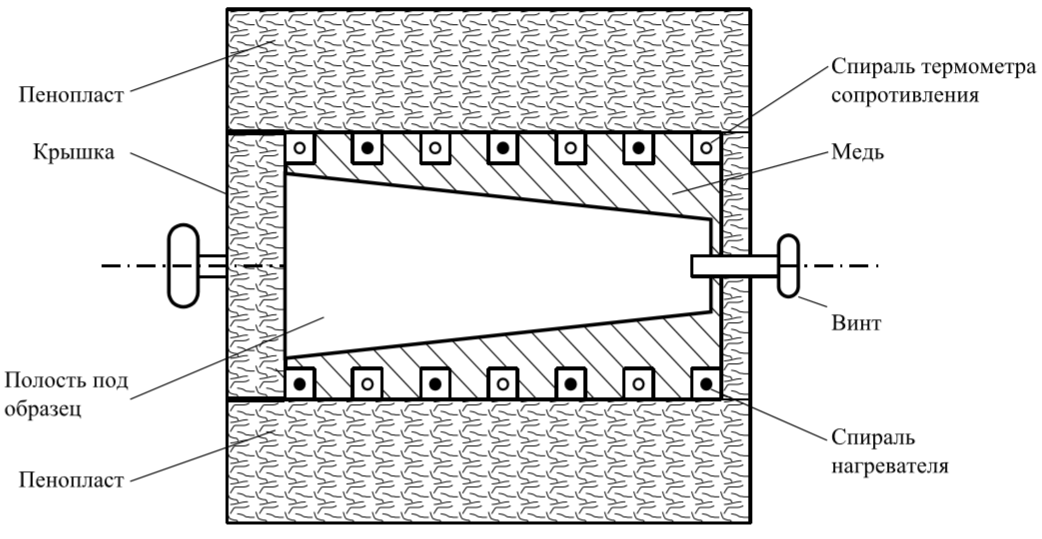
\includegraphics[width=0.8\textwidth]{pic1.png}
	\caption{Схема устройства калориметра}
	\label{fig:calorimeter}
\end{figure}

Температура измеряется термометром сопротивления, который представляет собой медную проволоку, намотанную на теплопроводящий каркас внутренней стенки калориметра (рис. 1). Сопротивление проводника изменяется с температурой по закону

\begin{equation}
    R_{T} = R_{0}(1 + \alpha \Delta T),
    \label{RT}
\end{equation}

где $R_{T}$ -- сопротивление термеметра про $T  ^{\circ}C$, $R_{0}$ -- его сопротивление при $0  ^{\circ}C$, $\alpha$ -- температурный коэффициент сопротивления. 

Дифференцируя (5) по времени, найдем

\begin{equation}
    \frac{dR}{dt} = R_{0}\alpha \frac{dT}{dt},
    \label{dRT}
\end{equation}

Выразим сопротивление $R_{0}$ через исмеренное значение $R_{\text{к}}$ -- сопротивление термометра при комнатной температуре. Согласно (5), имеем

\begin{equation}
    R_{0} = \frac{R_{\text{к}}}{1 + \alpha \Delta T_{\text{к}}},
    \label{R0}
\end{equation}

Подставляя (6) и (7) в (4), найдем

\begin{equation}
    C_к = \frac{PR_{\text{к}} \alpha}{(\frac{dR}{dt})_{T_{\text{к}}}(1 + \alpha \Delta T_{\text{к}})},
    \label{capacity}
\end{equation}
 
 Входящий в формулу температурный коэффициент сопротивления меди равен $\alpha = 4,28 \cdot 10^{-3}~\text{град}^{-1}$, все остальные величины определяются экспериментально.
 Таким образом, для определения удельной теплоемкости образцов, будем использовать
\begin{equation}
 C = \frac{P}{m\cdot(\frac{dR}{dt})_{T_{\text{к}}}}- \frac{С_к}{m}
 \end{equation}
 

\section{Экспериментальная установка}
 
Установка состоит из калориметра с пенопластовой изоляцией, помещенного в ящик из многослойной клееной фанеры. Внутренние стенки калориметра выполненым из материала с высокой теплопроводностью. Надежность теплового контакта между телом и стенками обеспечивается их формой: они имеют вид усеченных конусов и плотно прилегают друг к другу. В стенку калориметра вмонтированы электронагреватель и термометр сопротивления. Схема включения нагревателя изображения на рис.2. Система реостатов позволяет установить нужную силу тока в цепи нагревателя. По амперметру и вольтметру определяется мощность, выделяемая в нагревателе. Величина сопротивления термометра измеряется мостом постоянного тока.

\begin{figure}[!h]
	\centering
	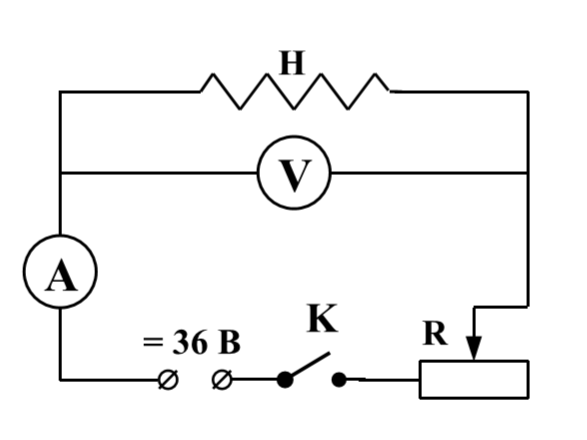
\includegraphics[width=0.4\textwidth]{pic2.png}
	\caption{Схема включения нагревателя}
	\label{fig:boiler}
\end{figure}

Зафиксируем параметры установки и образцов (напряжение и ток в термометре, мощность термометра, массы образцов):

$U = 36~\text{В},~ I = 0,3~\text{А},~ P = 10,8~\text{Вт}$
\begin{table}[!h]
	\centering
	\begin{tabular}{|l|l|l|l|}
		\hline
	& Железный образец	& Латунный образец & Алюминиевый образец \\ \hline
		Масса, г & $815,1\pm0,1$   & $875,5\pm0,1$      & $294,2\pm0,1$           \\ \hline
	\end{tabular}
\end{table}
 
\section{Обработка результатов измерений}
\begin{enumerate}

\item  Снимем зависимость $R(t)$ для калориметра, а также для 3 исследуемых образцов и построим графики зависимости $R(t)$ для результатов измерений.
\begin{figure}[h!]
    \centering
    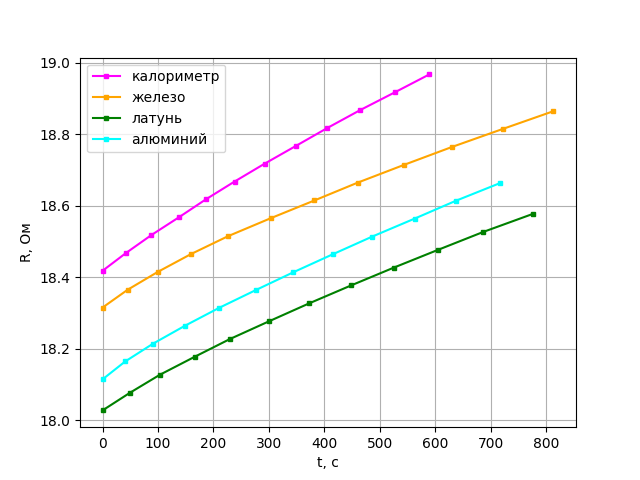
\includegraphics[scale=0.72]{R(t).png}
    \caption{Зависимость R(t)}
\end{figure}
\item  По полученным данным построим также графики зависимостей $\frac{dR}{dt} \left( R \right)$ для различных серий измерений, т.е. для калориметра и 3 исследуемых образцов. Данную зависимость построим с учетом формулы:
\begin{equation}
		\frac{dR}{dt} \left( R_{t_{1}} \right) = \frac{R_{t_{2}} - R_{t_{2}}}{t_{2} - t_{1}}
		\label{eq:derivates}
	\end{equation}

\begin{figure}[h!]
    \centering
    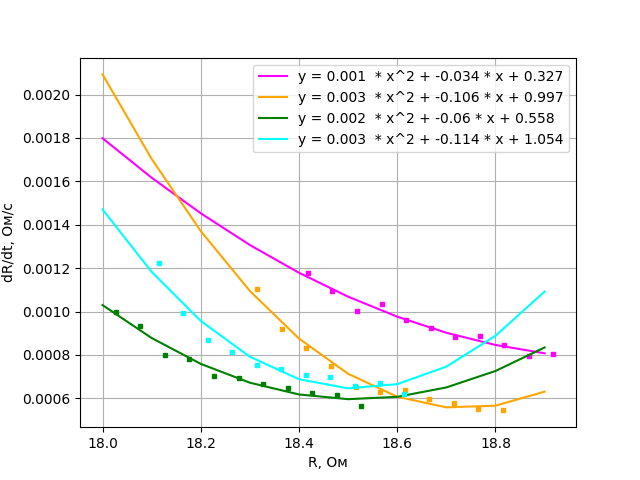
\includegraphics[scale=0.72]{dRdt(R).png}
    \caption{Зависимость dR/dt(R)}
\end{figure}

\item Экстраполируем полученные зависимости полиномом второй степени до значений $R = R_{\text{к}}$ и вычислим значения $(\frac{dR}{dt})_{T = T_{\text{к}}}$ с использованием полученной формулы.

\begin{table}[!h]
	\centering
	\begin{tabular}{|l|l|l|l|}
		\hline
		& Уравнение экстраполяции                     & $R_{\text{к}}$, Ом     & $(dR/dt)_{R_{\text{к}}} \cdot 10^{-4}$, Ом/с     \\ \hline
		Калориметр & $y = 0,001x^2 - 0,034x + 0,327$ & 18,105 & $16,08 \pm 0,12$ \\ \hline
		Железо     & $y = 0,003x^2 - 0,106x + 0,997$ & 18,105 & $16,85 \pm 0,16$ \\ \hline
		Латунь     & $y = 0,002x^2 - 0,06x + 0,558$  & 18,105 & $8,71 \pm 0,12$ \\ \hline
		Алюминий   & $y = 0,003x^2 - 0,114x + 1,054$ & 18,105 & $11,70 \pm 0,22$ \\ \hline
		
	\end{tabular}
	\caption{Экстраполяция}
\end{table}
\item Вычисляем, используя полученные зависимости при экстраполяции теплоемкость калориметра по формуле (6), суммарную теплоемкость образцов с калориметром по формуле (4) и удельную теплоемкость образцов по формуле (9). Для определения погрешностей косвенных измерений, учтем, что погрешности измерения сопротивления мостом, массы образцов весами и времени секундомером, а также случайные погрешности,  крайне малы в сравнении с погрешностью экстраполяции функций. Вследствие этого, для расчета погрешности определяемых величин, ограничемся рассмотрением вклада только последней.


\begin{table}[!h]
	\begin{center}
		\scalebox{0.85}{
		\begin{tabular}{|l|l|l|l|}
			\hline
			& Теплоемкость, Дж/К & Тепл. без калориметра, Дж/К & Удельная тепл., Дж/кг$\cdot$К \\ \hline
			Калориметр & $897 \pm 7$  & -                            & -                     \\ \hline
			Железный  образец   & $1238 \pm 11$  & $341 \pm 13$                  & $418 \pm 16$          \\ \hline
			Латунный образец     & $1180 \pm 15$  & $283 \pm 17 $                & $323 \pm 20$           \\ \hline
			Алюминиевый образец   & $1092 \pm 21$  & $195 \pm 22$                  & $663 \pm 74$           \\ \hline
		\end{tabular}}
	\end{center}
	\caption{Результат вычислений теплоемкости}
\end{table}

\end{enumerate}

	

\section{Вывод}

	\item В ходе работы были измерены удельные теплоемкости железа, латуни и алюминия: $c_{\text{железо}} = 418\pm 16 \frac{\text{Дж}}{\text{кг}\cdot\text{К}}$,~$c_{\text{латунь}} = 323\pm 20 \frac{\text{Дж}}{\text{кг}\cdot\text{К}}$,~ $c_{\text{алюминий}} = 663\pm 74 \frac{\text{Дж}}{\text{кг}\cdot\text{К}}$. Табличные значения для этих матриалов: $c^{\text{табл.}}_{\text{железо}} = 460 \frac{\text{Дж}}{\text{кг}\cdot\text{К}}$ $c^{\text{табл.}}_{\text{латунь}} = 380 \frac{\text{Дж}}{\text{кг}\cdot\text{К}}$,  и $c^{\text{табл.}}_{\text{алюминий}} = 920 \frac{\text{Дж}}{\text{кг}\cdot\text{К}}$. В пределах погрешности значения теплоемкости для образцов из железа и латуни хорошо сходятся с табличными данными, но вот значение теплоемкости алюминия отличается значительно, несмотря даже на то, что диапазон погрешностей достаточно велик в данном эксперименте. Причиной такого результата может являться, во-первых, то, что теплоемкость алюмния значительно выше, чем у других исследуемых материалов, вследствие чего процесс нагревания и охлаждения в этом образце происходит с большей скоростью, что ведет к большей разнице температур с окружающим пространством, и, следовательно, к большим тепловым потерям за время проведения эксперимента (формула (3)). С учетом этого, наша зависимость $R(t)$ и полученный из нее график $\frac{dR}{dt} \left( R \right)$ для экстраполяции значения $(\frac{dR}{dt})_{T = T_{\text{к}}}$ не вполне соответствуют действительности. Во-вторых, отличие полученной удельной теплоемкости алюминия от табличного значения может быть связано с чистотой исследуемого образца: образец представляет собой сплав металлов неизвестного процентного состава, вследствие чего его удельная теплоемкость не являетя удельной теплоемкостью чистого  алюминия (это замечание также относится и к образцам для исследования удельной теплоемкости железа и латуни). 


\end{document}
